% --- Aufgabenblatt: Schrägbilder zeichnen (7. Klasse) ---

\section*{Aufgabenblatt: Schrägbilder zeichnen}

\subsection*{1. Grundlagen}
\textbf{a)} Erkläre, was ein Schrägbild ist und wozu es verwendet wird.

\textbf{b)} Welche Regeln gelten beim Zeichnen von Schrägbildern (z.B. Verzerrungsfaktor, Winkel)?

\subsection*{2. Quader als Schrägbild}
\textbf{a)} Zeichne ein Schrägbild eines Quaders mit den Kantenlängen $a=5\,\mathrm{cm}$, $b=3\,\mathrm{cm}$, $c=2\,\mathrm{cm}$. Verwende einen Verzerrungsfaktor von $0{,}5$ und einen Schrägwinkel von $45^\circ$. Markiere die Vorderkante und beschrifte die Kanten.

\subsection*{3. Schrägbild eines Würfels}
\textbf{a)} Zeichne ein Schrägbild eines Würfels mit der Kantenlänge $4\,\mathrm{cm}$ (Verzerrungsfaktor $0{,}5$, Schrägwinkel $45^\circ$). Markiere die Vorderfläche farbig und beschrifte die Kanten.

\subsection*{4. Schrägbild einer quadratischen Pyramide}
\textbf{a)} Zeichne ein Schrägbild einer quadratischen Pyramide mit Grundkante $4\,\mathrm{cm}$ und Höhe $5\,\mathrm{cm}$.

\subsection*{5. Anwendungsaufgaben}
\textbf{a)} Ein Karton hat die Maße $6\,\mathrm{cm} \times 4\,\mathrm{cm} \times 2\,\mathrm{cm}$. Fertige ein Schrägbild an und beschrifte die Maße.

\textbf{b)} Ein Aquarium ist ein Quader mit $8\,\mathrm{cm} \times 5\,\mathrm{cm} \times 3\,\mathrm{cm}$. Zeichne ein Schrägbild und markiere die Wasseroberfläche (halb voll).

\subsection*{6. Knobelaufgabe}
\textbf{a)} Überlege dir selbst einen Körper (z.B. L-förmiger Quader) und fertige ein Schrägbild davon an. Beschrifte die Kanten.

\newpage

% --- Karierte Zeichenfläche für Schrägbilder ---

\section*{Zeichenfläche für Schrägbilder}

\begin{center}
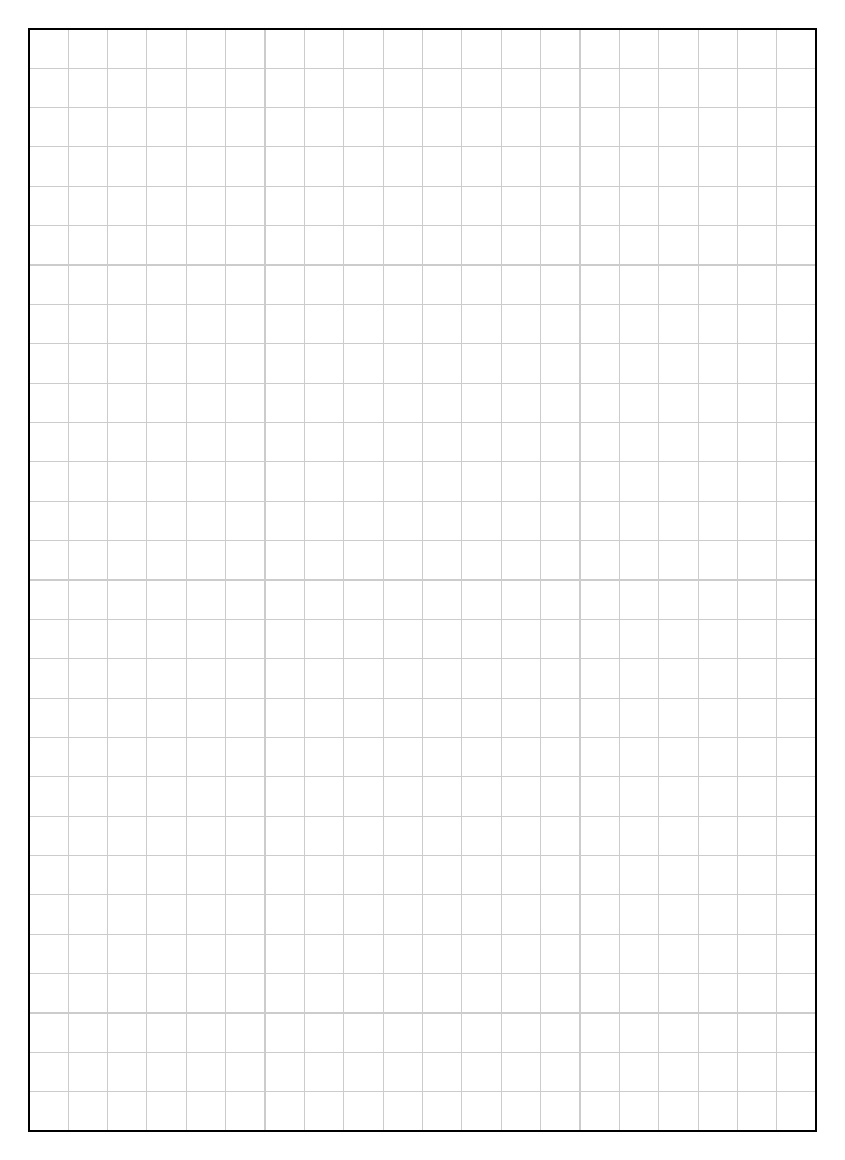
\begin{tikzpicture}[scale=0.5]
  % Karos zeichnen (20x28)
  \foreach \x in {0,...,20} {
    \draw[gray!40, thin] (\x,0) -- (\x,28);
  }
  \foreach \y in {0,...,28} {
    \draw[gray!40, thin] (0,\y) -- (20,\y);
  }
  % Rahmen
  \draw[black, thick] (0,0) rectangle (20,28);
\end{tikzpicture}
\end{center}

\vspace{1cm}

\begin{center}
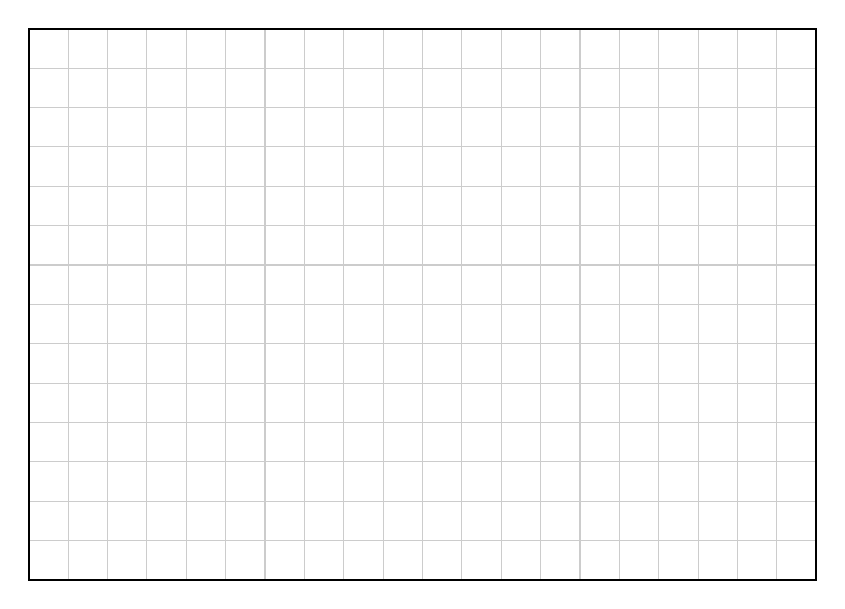
\begin{tikzpicture}[scale=0.5]
  % Karos zeichnen (20x14)
  \foreach \x in {0,...,20} {
    \draw[gray!40, thin] (\x,0) -- (\x,14);
  }
  \foreach \y in {0,...,14} {
    \draw[gray!40, thin] (0,\y) -- (20,\y);
  }
  % Rahmen
  \draw[black, thick] (0,0) rectangle (20,14);
\end{tikzpicture}
\end{center}

% --- Ende des Aufgabenblatts ---
